\chapter{Actual Outcome}
        \section{Data Collection Results}
        The data collection phase successfully extracted data from all three sources:

        \subsection{Energy Data from NEA Reports}
        \begin{itemize}
            \item \textbf{PDF Files Processed:} 18 NMOR reports (2079/04 to 2080/11)
            \item \textbf{Daily Energy Records:} 606 records extracted
            \item \textbf{Peak Demand Records:} 604 records extracted
            \item \textbf{Date Range:} July 17, 2022 to March 13, 2024
            \item \textbf{Variables Captured:} 12 columns per daily record
        \end{itemize}

        \subsection{Weather Data}
        \begin{itemize}
            \item \textbf{Cities:} Kathmandu and Pokhara
            \item \textbf{Hourly Records:} 24,864 records
            \item \textbf{Daily Aggregated Records:} 518 days
            \item \textbf{Variables:} Temperature, humidity, precipitation, wind speed
            \item \textbf{Period:} July 2022 to November 2023
        \end{itemize}

        \subsection{Holiday Calendar}
        \begin{itemize}
            \item \textbf{Holidays Compiled:} 30 dates for 2022-2024
            \item \textbf{Types:} National, Festival, International
        \end{itemize}

        \section{Exploratory Data Analysis Results}
        The EDA revealed significant patterns in Nepal's energy consumption:

        \subsection{Energy Demand Statistics}
        \begin{table}[h]
                \begin{center}
                \begin{tabular}{|l|r|}
                \hline
                \textbf{Metric} & \textbf{Value} \\
                \hline
                Mean Daily Demand & 32,191 MWh \\
                \hline
                Maximum Demand & 42,190 MWh \\
                \hline
                Minimum Demand & 18,936 MWh \\
                \hline
                Standard Deviation & 4,613 MWh \\
                \hline
                \end{tabular}
                \end{center}
                \caption{Energy Demand Statistics}
        \end{table}

        \subsection{Seasonal Patterns}
        \begin{itemize}
            \item \textbf{Highest Demand:} Summer months (May-July) due to cooling needs
            \item \textbf{Lowest Demand:} Spring months (March-April) with mild weather
            \item \textbf{Festival Impact:} Noticeable changes during Dashain and Tihar
        \end{itemize}

        \subsection{Generation Mix Analysis}
        \begin{table}[h]
                \begin{center}
                \begin{tabular}{|l|r|r|}
                \hline
                \textbf{Source} & \textbf{Avg Contribution (MWh)} & \textbf{Share} \\
                \hline
                IPP & 16,464 & 43\% \\
                \hline
                NEA Subsidiary & 7,180 & 30\% \\
                \hline
                NEA Own Generation & 7,935 & 23\% \\
                \hline
                Import from India & 4,607 & 4\% \\
                \hline
                \end{tabular}
                \end{center}
                \caption{Average Daily Energy by Source}
        \end{table}

        \begin{figure}[h]
                \centering
                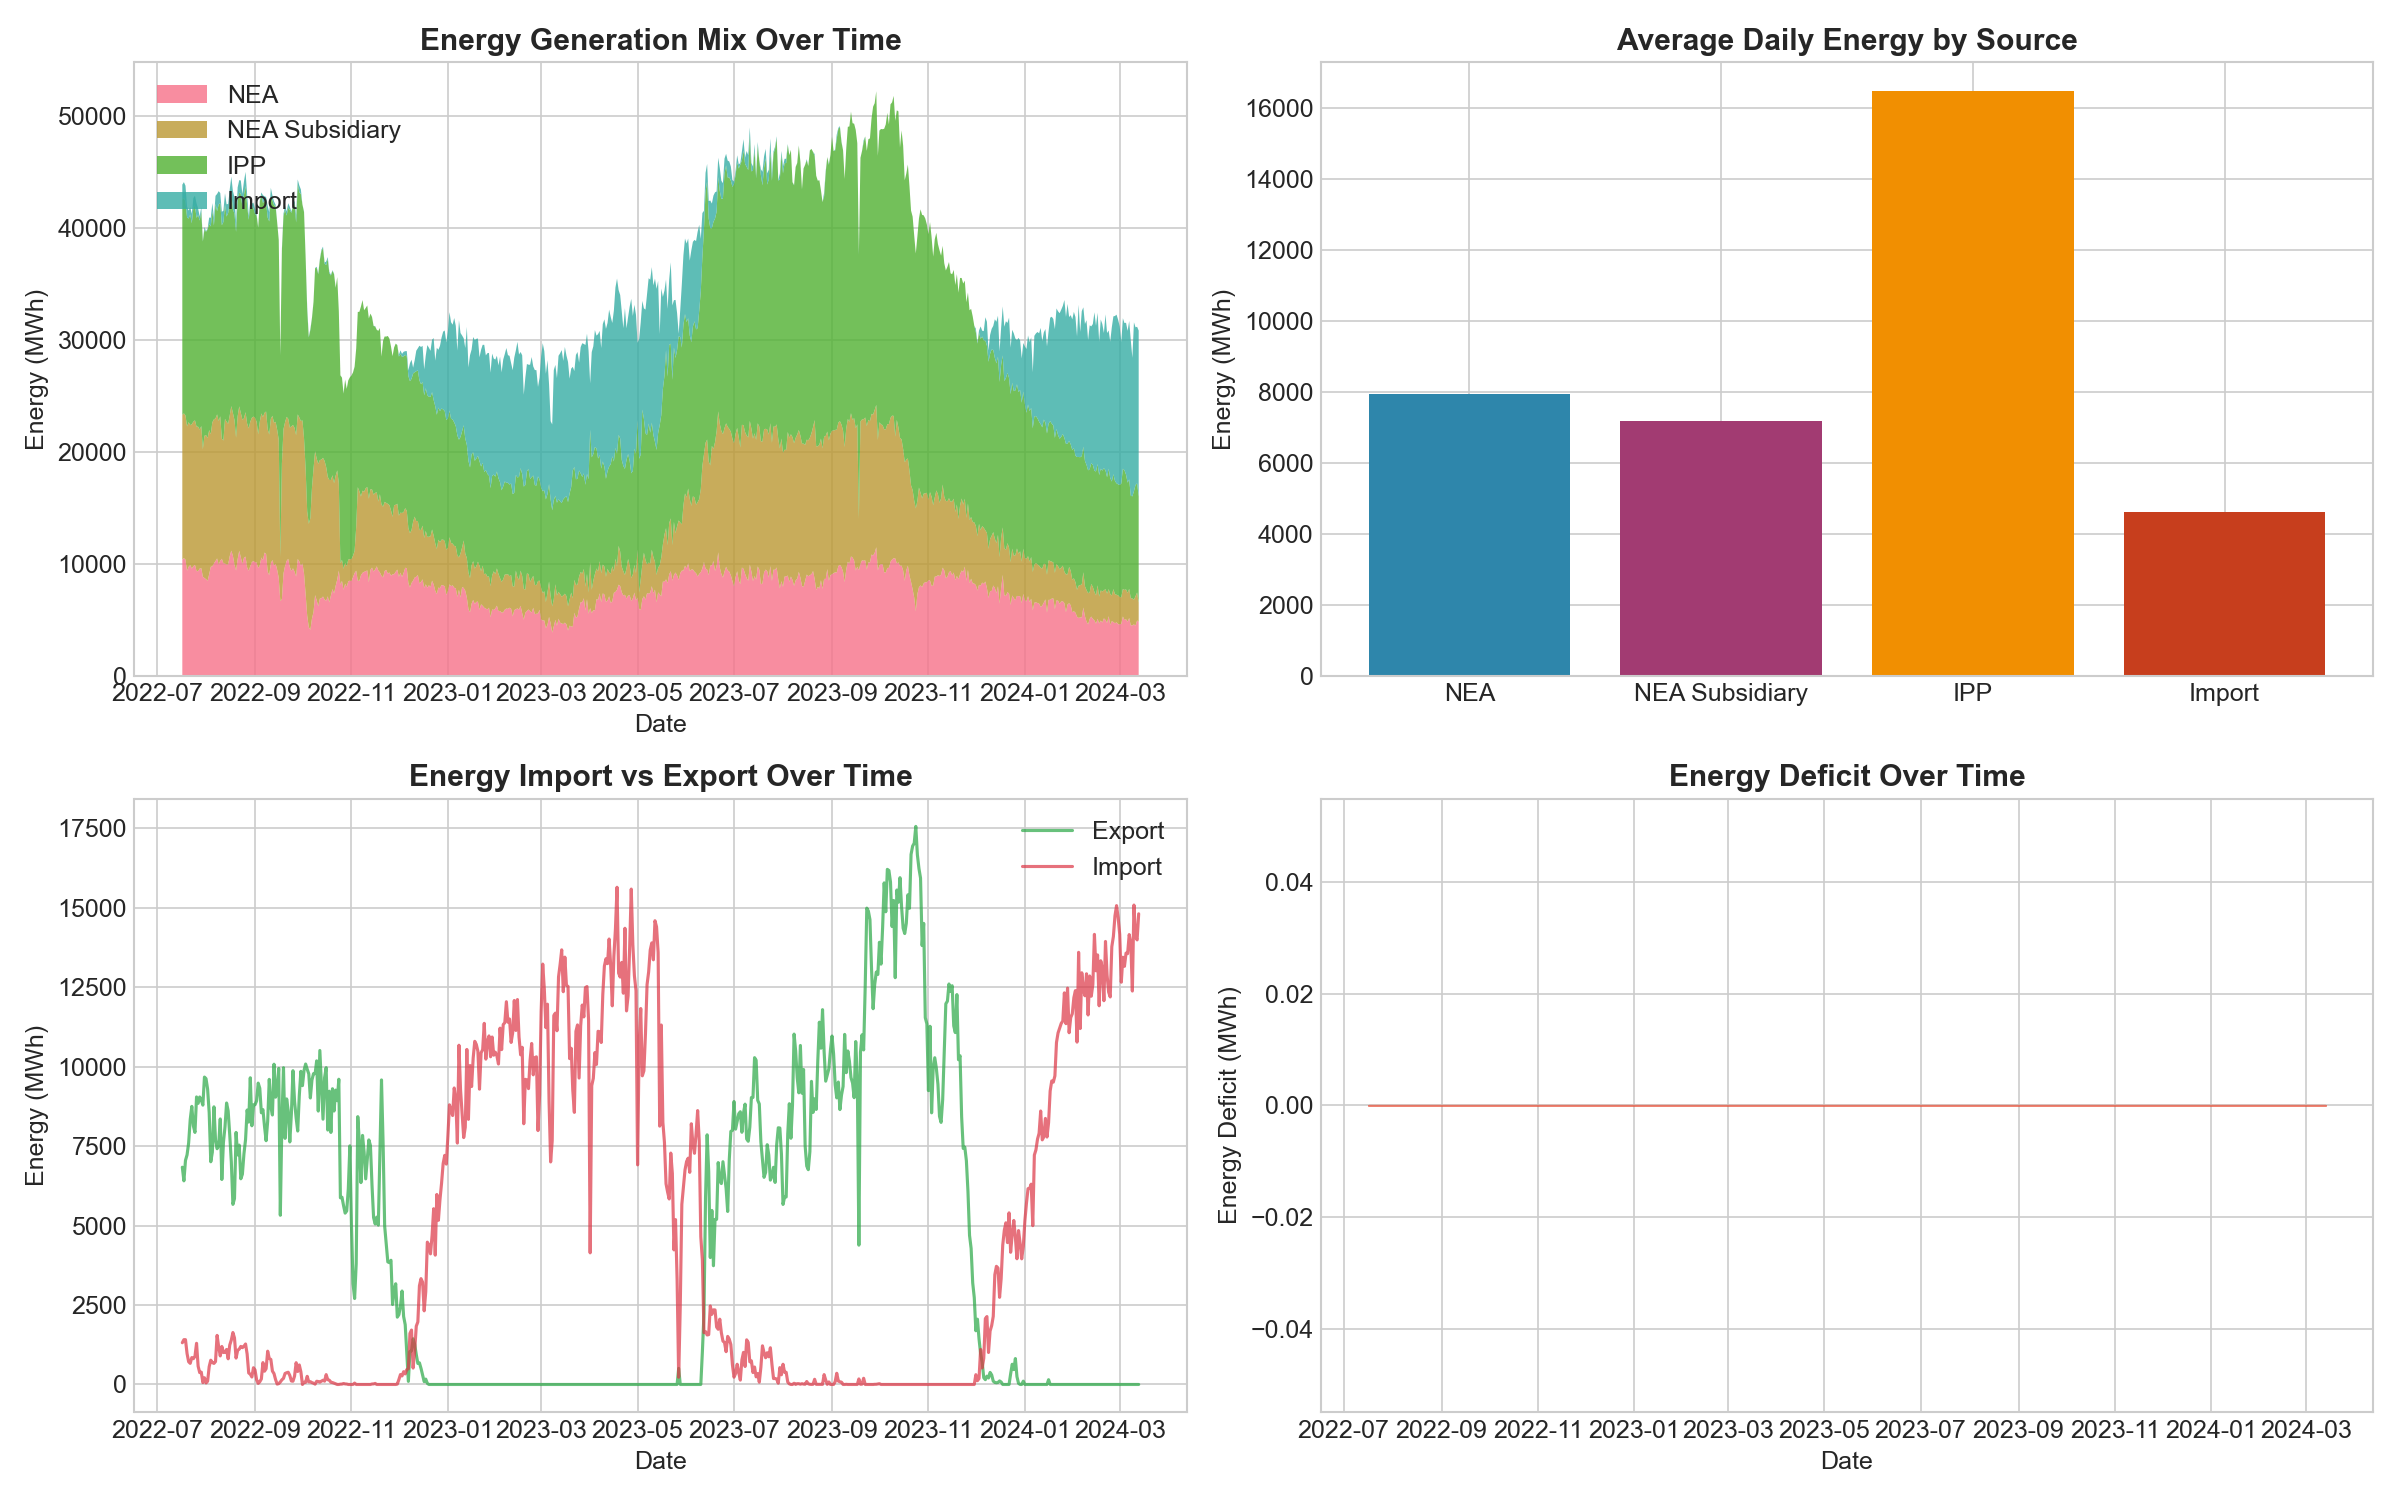
\includegraphics[width=0.9\textwidth]{img/generation_analysis.png}
                \caption{Energy Generation Mix Analysis}
        \end{figure}
        \pagebreak

        \section{Feature Engineering Results}
        The final dataset after feature engineering contained:

        \begin{itemize}
            \item \textbf{Total Records:} 495 (after dropping NaN from lag features)
            \item \textbf{Features:} 18 predictive features
            \item \textbf{Target:} Energy Requirement (MWh)
            \item \textbf{Training Set:} 396 samples (80\%)
            \item \textbf{Test Set:} 99 samples (20\%)
        \end{itemize}

        \section{Model Training and Evaluation Results}
        Four models were trained and evaluated on the test dataset:

        \begin{table}[h]
                \begin{center}
                \begin{tabular}{|l|r|r|r|r|}
                \hline
                \textbf{Model} & \textbf{Test RMSE} & \textbf{Test MAE} & \textbf{Test MAPE} & \textbf{Test R$^2$} \\
                \hline
                Ridge Regression & 1,660.94 & 1,324.15 & 4.32\% & 0.8991 \\
                \hline
                Linear Regression & 1,662.57 & 1,328.28 & 4.34\% & 0.8989 \\
                \hline
                Random Forest & 1,760.68 & 1,396.45 & 4.55\% & 0.8866 \\
                \hline
                XGBoost & 1,964.87 & 1,594.81 & 5.06\% & 0.8588 \\
                \hline
                \end{tabular}
                \end{center}
                \caption{Model Performance Comparison}
        \end{table}

        \begin{figure}[h]
                \centering
                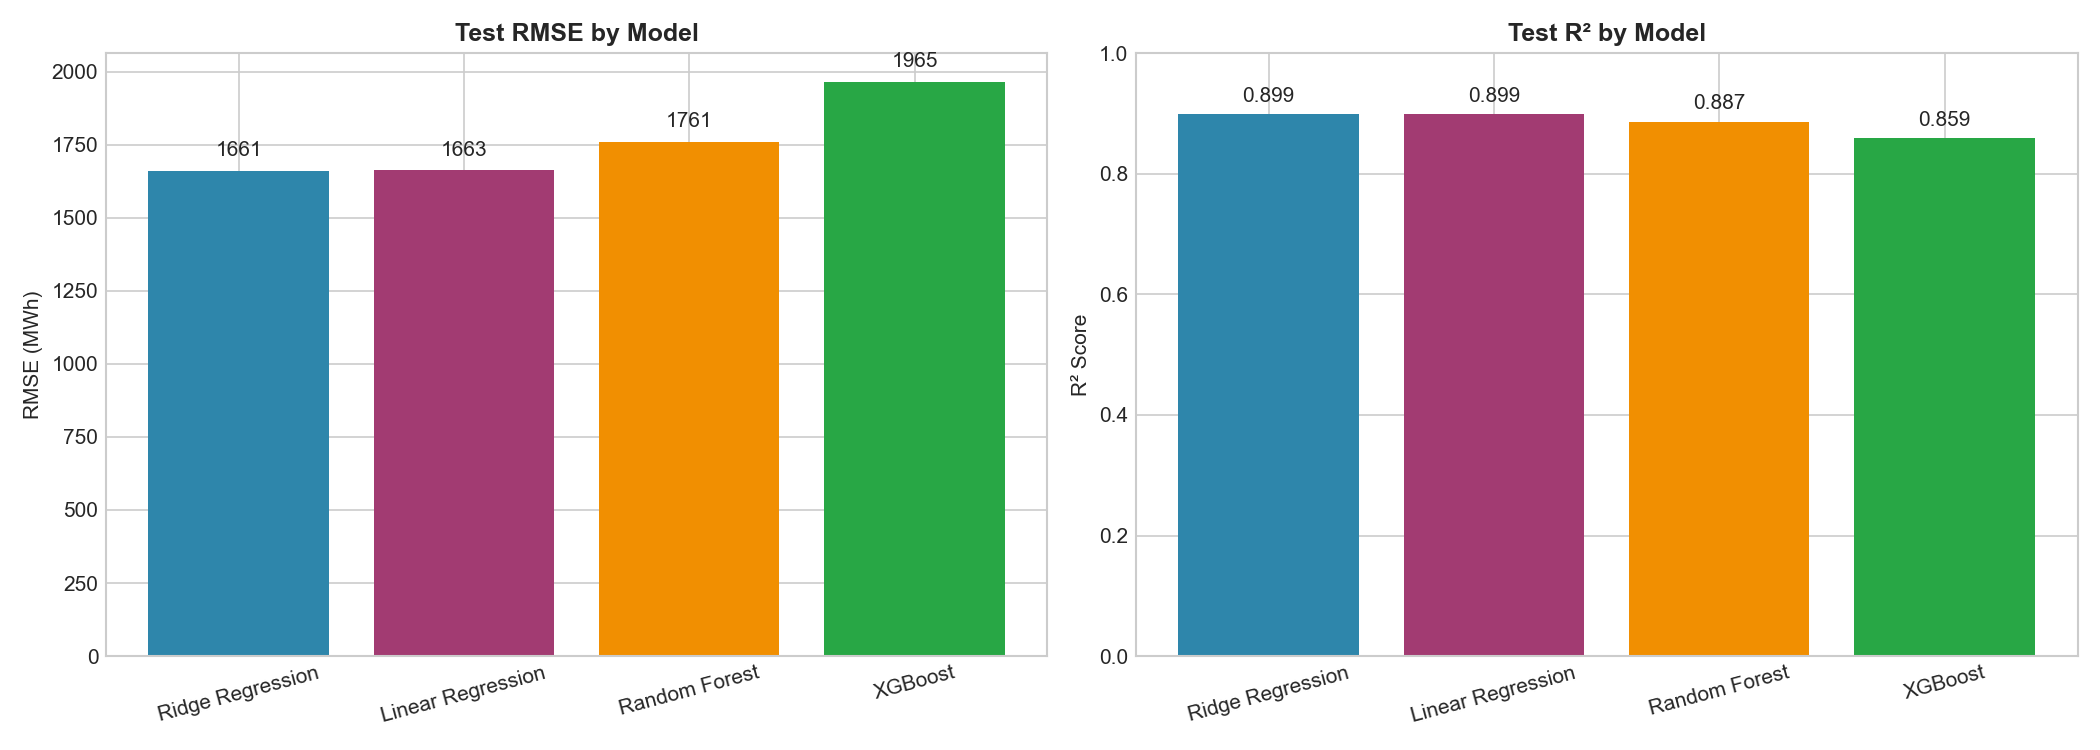
\includegraphics[width=0.9\textwidth]{img/model_comparison.png}
                \caption{Model Comparison - RMSE and R$^2$}
        \end{figure}
        \pagebreak

        \section{Best Model Analysis}
        \subsection{Selected Model: Ridge Regression}
        The Ridge Regression model achieved the best performance:
        \begin{itemize}
            \item \textbf{Test R$^2$:} 0.8991 (89.91\% variance explained)
            \item \textbf{Test RMSE:} 1,660.94 MWh
            \item \textbf{Test MAE:} 1,324.15 MWh
            \item \textbf{Test MAPE:} 4.32\%
        \end{itemize}

        \subsection{Why Ridge Outperformed Tree-Based Models}
        \begin{itemize}
            \item \textbf{Dataset Size:} 495 records is relatively small for complex models
            \item \textbf{Feature Linearity:} Energy demand has strong linear relationships with lag features
            \item \textbf{Regularization:} Ridge's L2 penalty prevented overfitting
            \item \textbf{Tree Overfitting:} Random Forest and XGBoost showed signs of overfitting (low train RMSE, higher test RMSE)
        \end{itemize}

        \subsection{Actual vs Predicted Visualization}
        \begin{figure}[h]
                \centering
                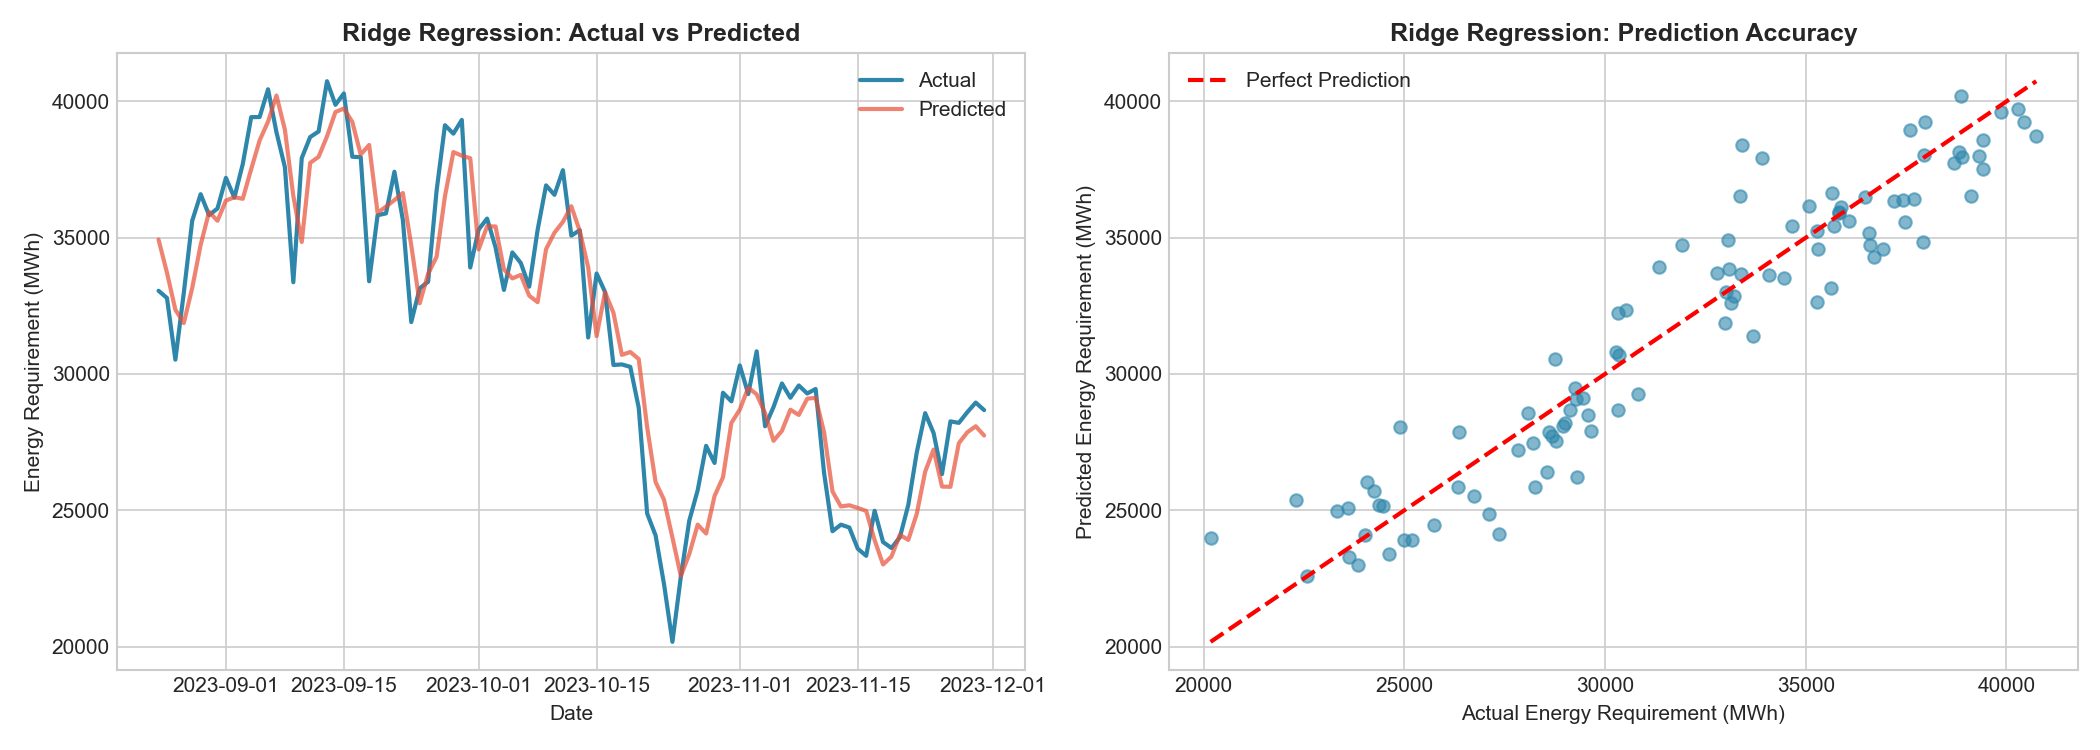
\includegraphics[width=0.95\textwidth]{img/prediction_results.png}
                \caption{Ridge Regression: Actual vs Predicted Energy Demand}
        \end{figure}
        \pagebreak

        \subsection{Residual Analysis}
        \begin{figure}[h]
                \centering
                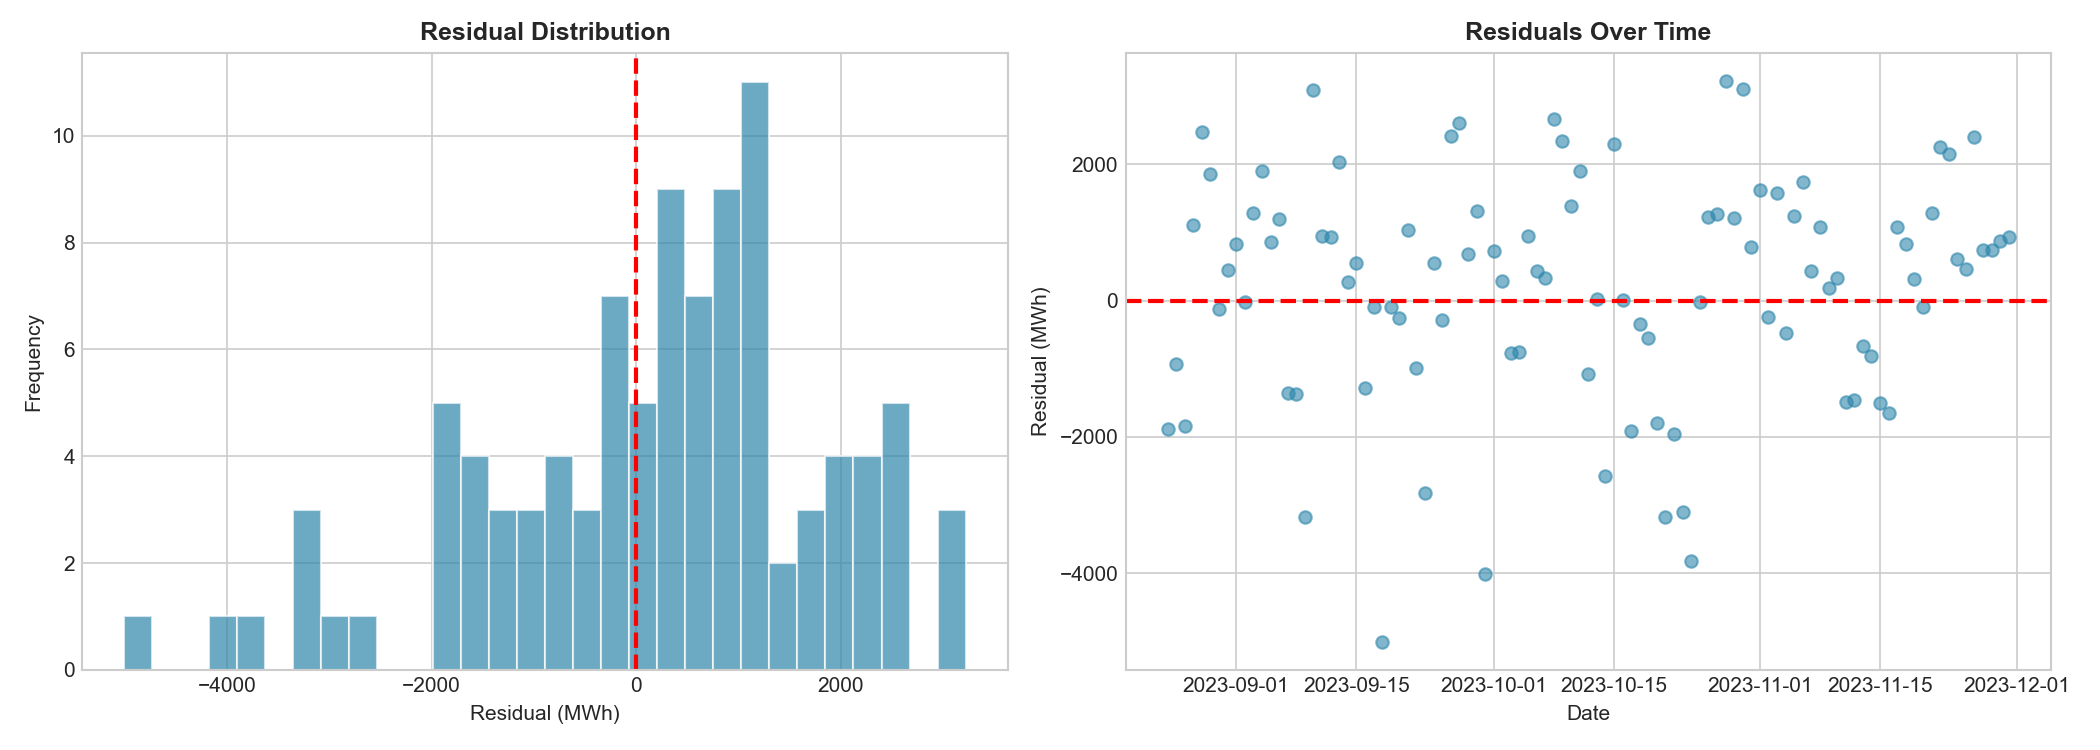
\includegraphics[width=0.95\textwidth]{img/residual_analysis.png}
                \caption{Residual Distribution and Analysis}
        \end{figure}

        \textbf{Residual Statistics:}
        \begin{itemize}
            \item Mean: Near 0 MWh (unbiased predictions)
            \item Standard Deviation: $\sim$1,600 MWh
            \item Range: -4,500 to +4,200 MWh
        \end{itemize}

        \section{Sample Predictions}
        \begin{table}[h]
                \begin{center}
                \begin{tabular}{|c|r|r|r|}
                \hline
                \textbf{Date} & \textbf{Actual (MWh)} & \textbf{Predicted (MWh)} & \textbf{Error (\%)} \\
                \hline
                2023-08-24 & 33,052 & 34,930 & -5.68\% \\
                \hline
                2023-08-25 & 32,788 & 33,717 & -2.83\% \\
                \hline
                2023-08-26 & 30,524 & 32,357 & -6.01\% \\
                \hline
                2023-08-27 & 32,978 & 31,868 & +3.36\% \\
                \hline
                2023-08-28 & 35,623 & 33,159 & +6.92\% \\
                \hline
                \end{tabular}
                \end{center}
                \caption{Sample Predictions from Test Set}
        \end{table}

        \section{Key Insights}
        \subsection{Feature Importance}
        The analysis revealed that lag features are the most important predictors:
        \begin{enumerate}
            \item \textbf{demand\_rolling\_7:} 7-day moving average - captures medium-term trend
            \item \textbf{demand\_lag\_1:} Previous day's demand - captures short-term momentum
            \item \textbf{demand\_lag\_7:} Same day last week - captures weekly seasonality
            \item \textbf{temp\_mean:} Temperature - affects heating/cooling demand
            \item \textbf{day\_of\_week:} Weekly pattern
        \end{enumerate}

        \subsection{Model Accuracy}
        The model achieves:
        \begin{itemize}
            \item 90\% variance explained (R$^2$ = 0.90)
            \item 4.3\% average error (MAPE)
            \item Suitable for operational planning and grid management
        \end{itemize}

        \section{Saved Model Artifacts}
        The following files were saved for future use:
        \begin{itemize}
            \item \texttt{models/best\_model.joblib} - Trained Ridge Regression model
            \item \texttt{models/scaler.joblib} - StandardScaler for feature normalization
        \end{itemize}